\subsection{Intro}

Before starting the explanation, we add a brief high level description of Quaternions, which are used in messages to represent orientations. Even a distinction between pose and position is done.

\textbf{Quaternion}: a different way to describe the orientation of a frame only. It's an alternative to Yaw, Pitch and Roll. A quaternion has four parameters: x, y, z, w. Pay attention, they are NOT a position vector.

\textbf{Position}: position of the robot in a 3D space.

\textbf{Pose}: position (3 DOF) + orientation (3 DOF).

In conclusion the pose has 6 D.O.F. which are: x, y, z, roll, pitch, yaw. Euler angles can be converted to quaternions, which are better. Transformation functions of ROS can do this conversion and the reverse one.

In addition, we put a scheme (\ref{fig:bicycle_vehicle}) of the principal parameters and variables  used for linearization.

\begin{figure}[h]
	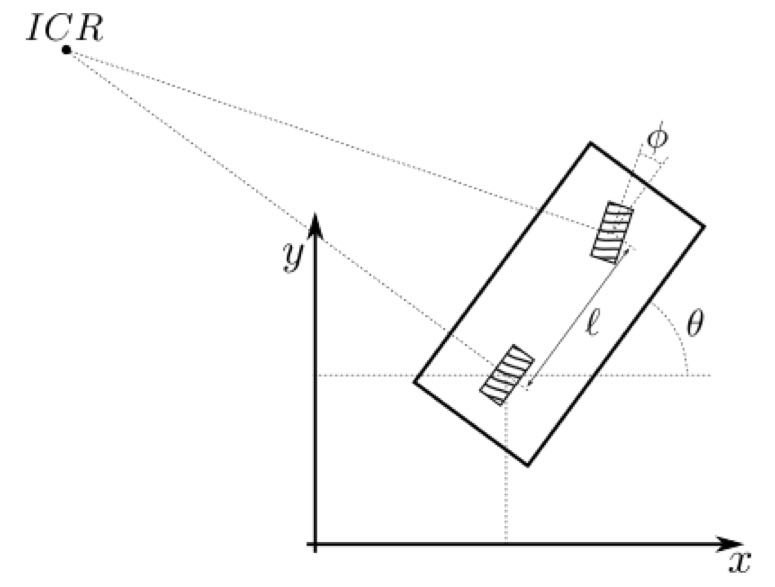
\includegraphics[scale=0.4]{kinematic_model}
	\caption{bicycle vehicle with main parameters and variables}
	\label{fig:bicycle_vehicle}
\end{figure}

\subsection{Configuration}

In the package there is a configuration file, containing: the parameter L, which represents distance between rear and front wheels; the parameter $\epsilon$, the distance between Center of Gravity and a point $P$, along the velocity vector. Linearization is done around point P. This parameter should be chosen empirically.

Both are used in the linearization.

\subsection{Launch}

There is a lunch file which \textbf{should be used to execute the node}. This contains also information about debugging level and loads configuration file.

\subsection{Node car\_kin\_linearizer}

\textbf{Node requirements}: distance between rear and front wheels as parameter.

The node has two callbacks:

\begin{itemize}
	\item One used to retrieve desired velocities of the point. These velocities are computed by trajectory tracker and published in \verb|/virtual_velocities| topic, subscribed by the controller node.
	\item One used to retrieve the orientation of the car around z axis. This is done reading from \verb|/vesc/odom|. The information retrieved are in the form of a quaternion and are converted into roll, pitch and yaw. Yaw is taken. In addition, even the speed around z axis is read (\verb|twist.angular.z|).
\end{itemize}

The node perform an exact linearization of the nonlinear bicycle cinematic model. The change of coordinates is applied as follows:

\[
V = V_{Xp}cos(\theta) + V_{Yp}sin(\theta)
\]

\[
\phi = \arctan\left(\frac{l}{\epsilon} \frac{ V_{Yp}cos(\theta) - V_{Xp}sin(\theta) }{ V_{Xp}cos(\theta) + V_{Yp}sin(\theta) }\right)
\]

Where 

\begin{itemize}
	\item $l$ is the distance between rear and front wheels
	\item $\epsilon$ is the distance between Center of Gravity and a point $P$
	\item $V_{Xp}$ and $V_{Yp}$ are the desired point velocities
	\item $\theta$ is the car orientation around z-axis
	\item $\phi$ is the steering angle
	\item $V$ is the driving velocity of the front wheel
\end{itemize}

In addition, the program compute the steering speed as $\omega = \frac{V}{l}\tan(\phi)$. This value is not used in the construction of the message because it's ignored by the model.

Once the linearization is performed an \verb|AckermannDriveStamped| message is built, containing $V$ and $\phi$. This message is published on \\ \verb|/vesc/ackermann_cmd_mux/input/navigation| topic, which is read by the model to make the car move. Linearization and command sending operations are repeated in a loop, which is the core of the node.